% Edge weights ell_e = log sin delta_e on the crossing graph and, at each label, in minus out, which is G_f = B ell.
% Source of the figure, typeset in the paper's own fonts (T1, Latin Modern, 11pt) at the paper's text
% width (6.5in), so \includegraphics does not rescale it. Illustrates CLH-2, CLH-4; it adds no assertion.
% Every coordinate and printed number is read from values that Lean evaluated (Conj43.crossEdges, Conj43.Bmat and the gradient);
% inputs: f-bar=(3,5,1,2,4), theta/pi=(0,0.1,0.7,0.3,0.8).
% SHA-256 (first 16 hex digits) of the output lines the values come from: inc 724ff4ada8b52bb2.
% Real-valued quantities are floating-point values computed in Lean from the paper's formulas.
% Build: pdflatex <this file> && pdftocairo -svg <this file>.pdf <this file>.svg
\documentclass[11pt]{standalone}
\usepackage[T1]{fontenc}
\usepackage{lmodern}
\usepackage{amsmath,amssymb}
\usepackage{tikz}
\usetikzlibrary{arrows.meta,positioning,calc}

% the palette of the paper's other figures: blue solid for the first curve or strand, ochre dashed for the second
\definecolor{ink}{HTML}{233740}
\definecolor{muted}{HTML}{65757D}
\definecolor{pblue}{HTML}{0072B2}
\definecolor{qochre}{HTML}{B87827}

\tikzset{
  frm/.style={draw=muted, line width=0.5pt},
  axl/.style={draw=muted!70, line width=0.4pt},
  crvP/.style={draw=pblue, line width=1.1pt, line join=round},
  crvQ/.style={draw=qochre, line width=1.1pt, dash pattern=on 4pt off 1.6pt},
  drop/.style={draw=muted, line width=0.4pt, dash pattern=on 1pt off 1.4pt},
  dotQ/.style={circle, fill=qochre, draw=qochre, inner sep=0pt, minimum size=4.2pt},
  dotP/.style={circle, fill=pblue, draw=pblue, inner sep=0pt, minimum size=4.2pt},
  openQ/.style={circle, fill=white, draw=qochre, line width=0.8pt, inner sep=0pt, minimum size=4.2pt},
  lab/.style={font=\footnotesize, inner sep=1.5pt, text=ink},
  labm/.style={font=\small, inner sep=1.5pt, text=ink},
  labQ/.style={font=\footnotesize, inner sep=1.5pt, text=qochre},
  labP/.style={font=\footnotesize, inner sep=1.5pt, text=pblue},
  tick/.style={font=\footnotesize, inner sep=1.2pt, text=muted},
  vtx/.style={circle, draw=ink, fill=white, line width=0.6pt, inner sep=0pt, minimum size=15pt, font=\small, text=ink},
  arrP/.style={pblue, line width=1.0pt, -{Stealth[length=5pt,width=4.2pt]}},
}

\begin{document}
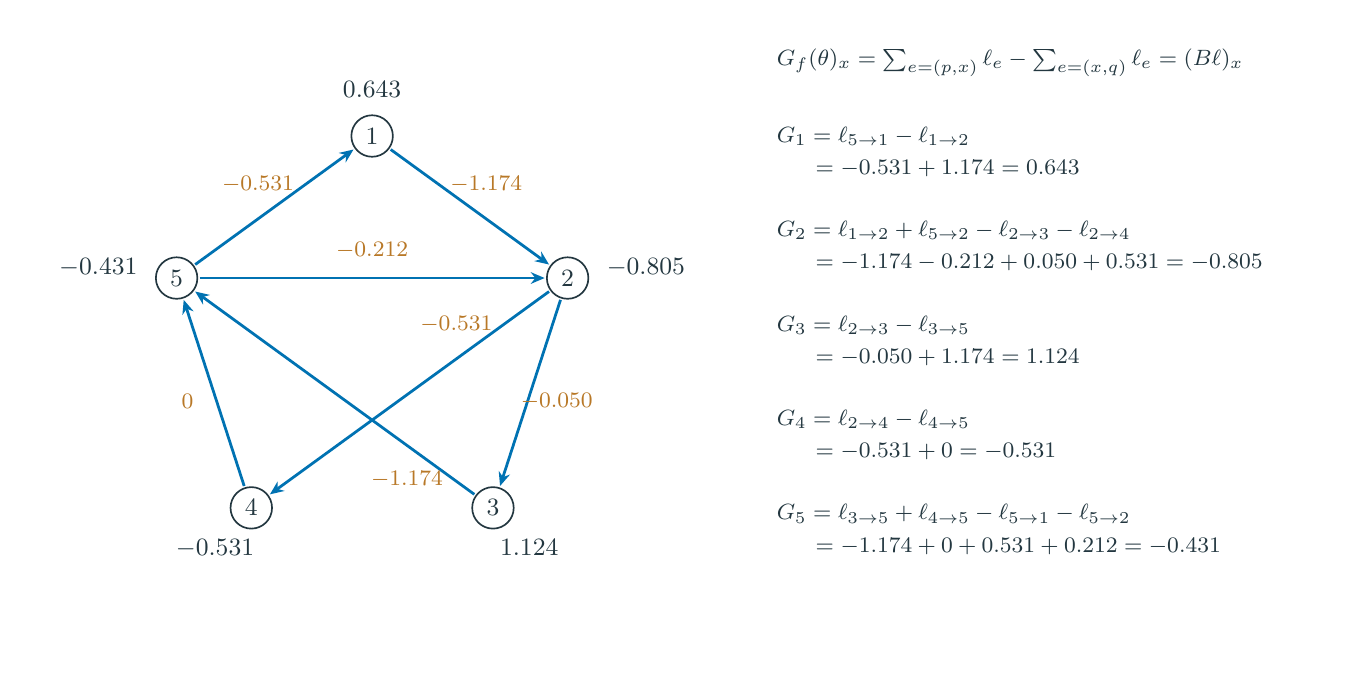
\begin{tikzpicture}[x=1bp,y=1bp]
\useasboundingbox (0,0) rectangle (468.005,225.0025);
\node[vtx] (v1) at (124.00,186.00) {1}; %mark C vertex 1
\node[vtx] (v2) at (194.38,134.87) {2}; %mark C vertex 2
\node[vtx] (v3) at (167.50,52.13) {3}; %mark C vertex 3
\node[vtx] (v4) at (80.50,52.13) {4}; %mark C vertex 4
\node[vtx] (v5) at (53.62,134.87) {5}; %mark C vertex 5
\draw[arrP, shorten >=0.5pt, shorten <=0.5pt] (v1) -- (v2); %c C 1,2
\node[labQ, anchor=center] at (165.07,168.52) {$-1.174$}; %val ell 0 -1.174
\draw[arrP, shorten >=0.5pt, shorten <=0.5pt] (v2) -- (v3); %c C 2,3
\node[labQ, anchor=center] at (190.45,90.41) {$-0.050$}; %val ell 1 -0.050
\draw[arrP, shorten >=0.5pt, shorten <=0.5pt] (v2) -- (v4); %c C 2,4
\node[labQ, anchor=center] at (154.34,118.14) {$-0.531$}; %val ell 2 -0.531
\draw[arrP, shorten >=0.5pt, shorten <=0.5pt] (v3) -- (v5); %c C 3,5
\node[labQ, anchor=center] at (136.57,62.24) {$-1.174$}; %val ell 3 -1.174
\draw[arrP, shorten >=0.5pt, shorten <=0.5pt] (v4) -- (v5); %c C 4,5
\node[labQ, anchor=center] at (57.55,90.41) {$0$}; %val ell 4 0
\draw[arrP, shorten >=0.5pt, shorten <=0.5pt] (v5) -- (v1); %c C 5,1
\node[labQ, anchor=center] at (82.93,168.52) {$-0.531$}; %val ell 5 -0.531
\draw[arrP, shorten >=0.5pt, shorten <=0.5pt] (v5) -- (v2); %c C 5,2
\node[labQ, anchor=center] at (124.00,144.87) {$-0.212$}; %val ell 6 -0.212
\node[labm, anchor=south] at (124.00,198.00) {$0.643$}; %val G 0 0.643
\node[labm, anchor=west] at (206.79,138.58) {$-0.805$}; %val G 1 -0.805
\node[labm, anchor=north] at (180.55,42.42) {$1.124$}; %val G 2 1.124
\node[labm, anchor=north] at (67.45,42.42) {$-0.531$}; %val G 3 -0.531
\node[labm, anchor=east] at (41.21,138.58) {$-0.431$}; %val G 4 -0.431
\node[lab, anchor=north west] at (268.00,219.00) {$G_f(\theta)_x=\sum_{e=(p,x)}\ell_e-\sum_{e=(x,q)}\ell_e=(B\ell)_x$};
\node[lab, anchor=north west] at (268.00,191.00) {$G_{1}=\ell_{5{\to}1}-\ell_{1{\to}2}$}; %val sym 1
\node[lab, anchor=north west] at (282.00,179.00) {$=-0.531+1.174=0.643$}; %val eq 1
\node[lab, anchor=north west] at (268.00,157.00) {$G_{2}=\ell_{1{\to}2}+\ell_{5{\to}2}-\ell_{2{\to}3}-\ell_{2{\to}4}$}; %val sym 2
\node[lab, anchor=north west] at (282.00,145.00) {$=-1.174-0.212+0.050+0.531=-0.805$}; %val eq 2
\node[lab, anchor=north west] at (268.00,123.00) {$G_{3}=\ell_{2{\to}3}-\ell_{3{\to}5}$}; %val sym 3
\node[lab, anchor=north west] at (282.00,111.00) {$=-0.050+1.174=1.124$}; %val eq 3
\node[lab, anchor=north west] at (268.00,89.00) {$G_{4}=\ell_{2{\to}4}-\ell_{4{\to}5}$}; %val sym 4
\node[lab, anchor=north west] at (282.00,77.00) {$=-0.531+0=-0.531$}; %val eq 4
\node[lab, anchor=north west] at (268.00,55.00) {$G_{5}=\ell_{3{\to}5}+\ell_{4{\to}5}-\ell_{5{\to}1}-\ell_{5{\to}2}$}; %val sym 5
\node[lab, anchor=north west] at (282.00,43.00) {$=-1.174+0+0.531+0.212=-0.431$}; %val eq 5
\end{tikzpicture}
\end{document}
